\documentclass[10pt]{beamer}

\usetheme{Madrid}
\usecolortheme{default}
\setbeamertemplate{navigation symbols}{}
\setbeamertemplate{footline}[frame number]

\usepackage[utf8]{inputenc}
\usepackage[T1]{fontenc}
\usepackage{lmodern}
\usepackage{amsmath}
\usepackage{amssymb}
\usepackage{graphicx}
\usepackage{booktabs}
\usepackage{listings}
\usepackage{xcolor}

\lstdefinestyle{pseudo}{
  basicstyle=\ttfamily\tiny,
  breaklines=true,
  columns=fullflexible,
  commentstyle=\color{teal},
}

\title[F2 $\tan(x)$ -- D1]{A User-Centred, From-Scratch Scientific Calculator\\ for the Tangent Function $\tan(x)$}
\subtitle{Deliverable 1: Persona, Requirements, Algorithms, CLI Prototype}
\author{Risat Ahmed \\ \small Student ID: 40294116}
\institute{SOEN 6011 -- Software Engineering Processes, Section CC \\ Concordia University -- Summer 2026}
\date{July 15, 2026}

\begin{document}

\begin{frame}
  \titlepage
\end{frame}

\begin{frame}{Outline}
  \tableofcontents
\end{frame}

\section{Persona}
\begin{frame}{Problem 1 --- Persona: Template Selection}
  \begin{columns}
    \begin{column}{0.5\textwidth}
      Three template styles compared: goal-directed, role-based, lightweight/proto-persona.

      \textbf{Selected: goal-directed} --- ties every persona field to a later requirement, matching a single-function calculator's design.

      \vspace{0.3cm}
      Role-based rejected: too heavy for one function. Lightweight rejected: too thin on traceability.
    \end{column}
    \begin{column}{0.5\textwidth}
      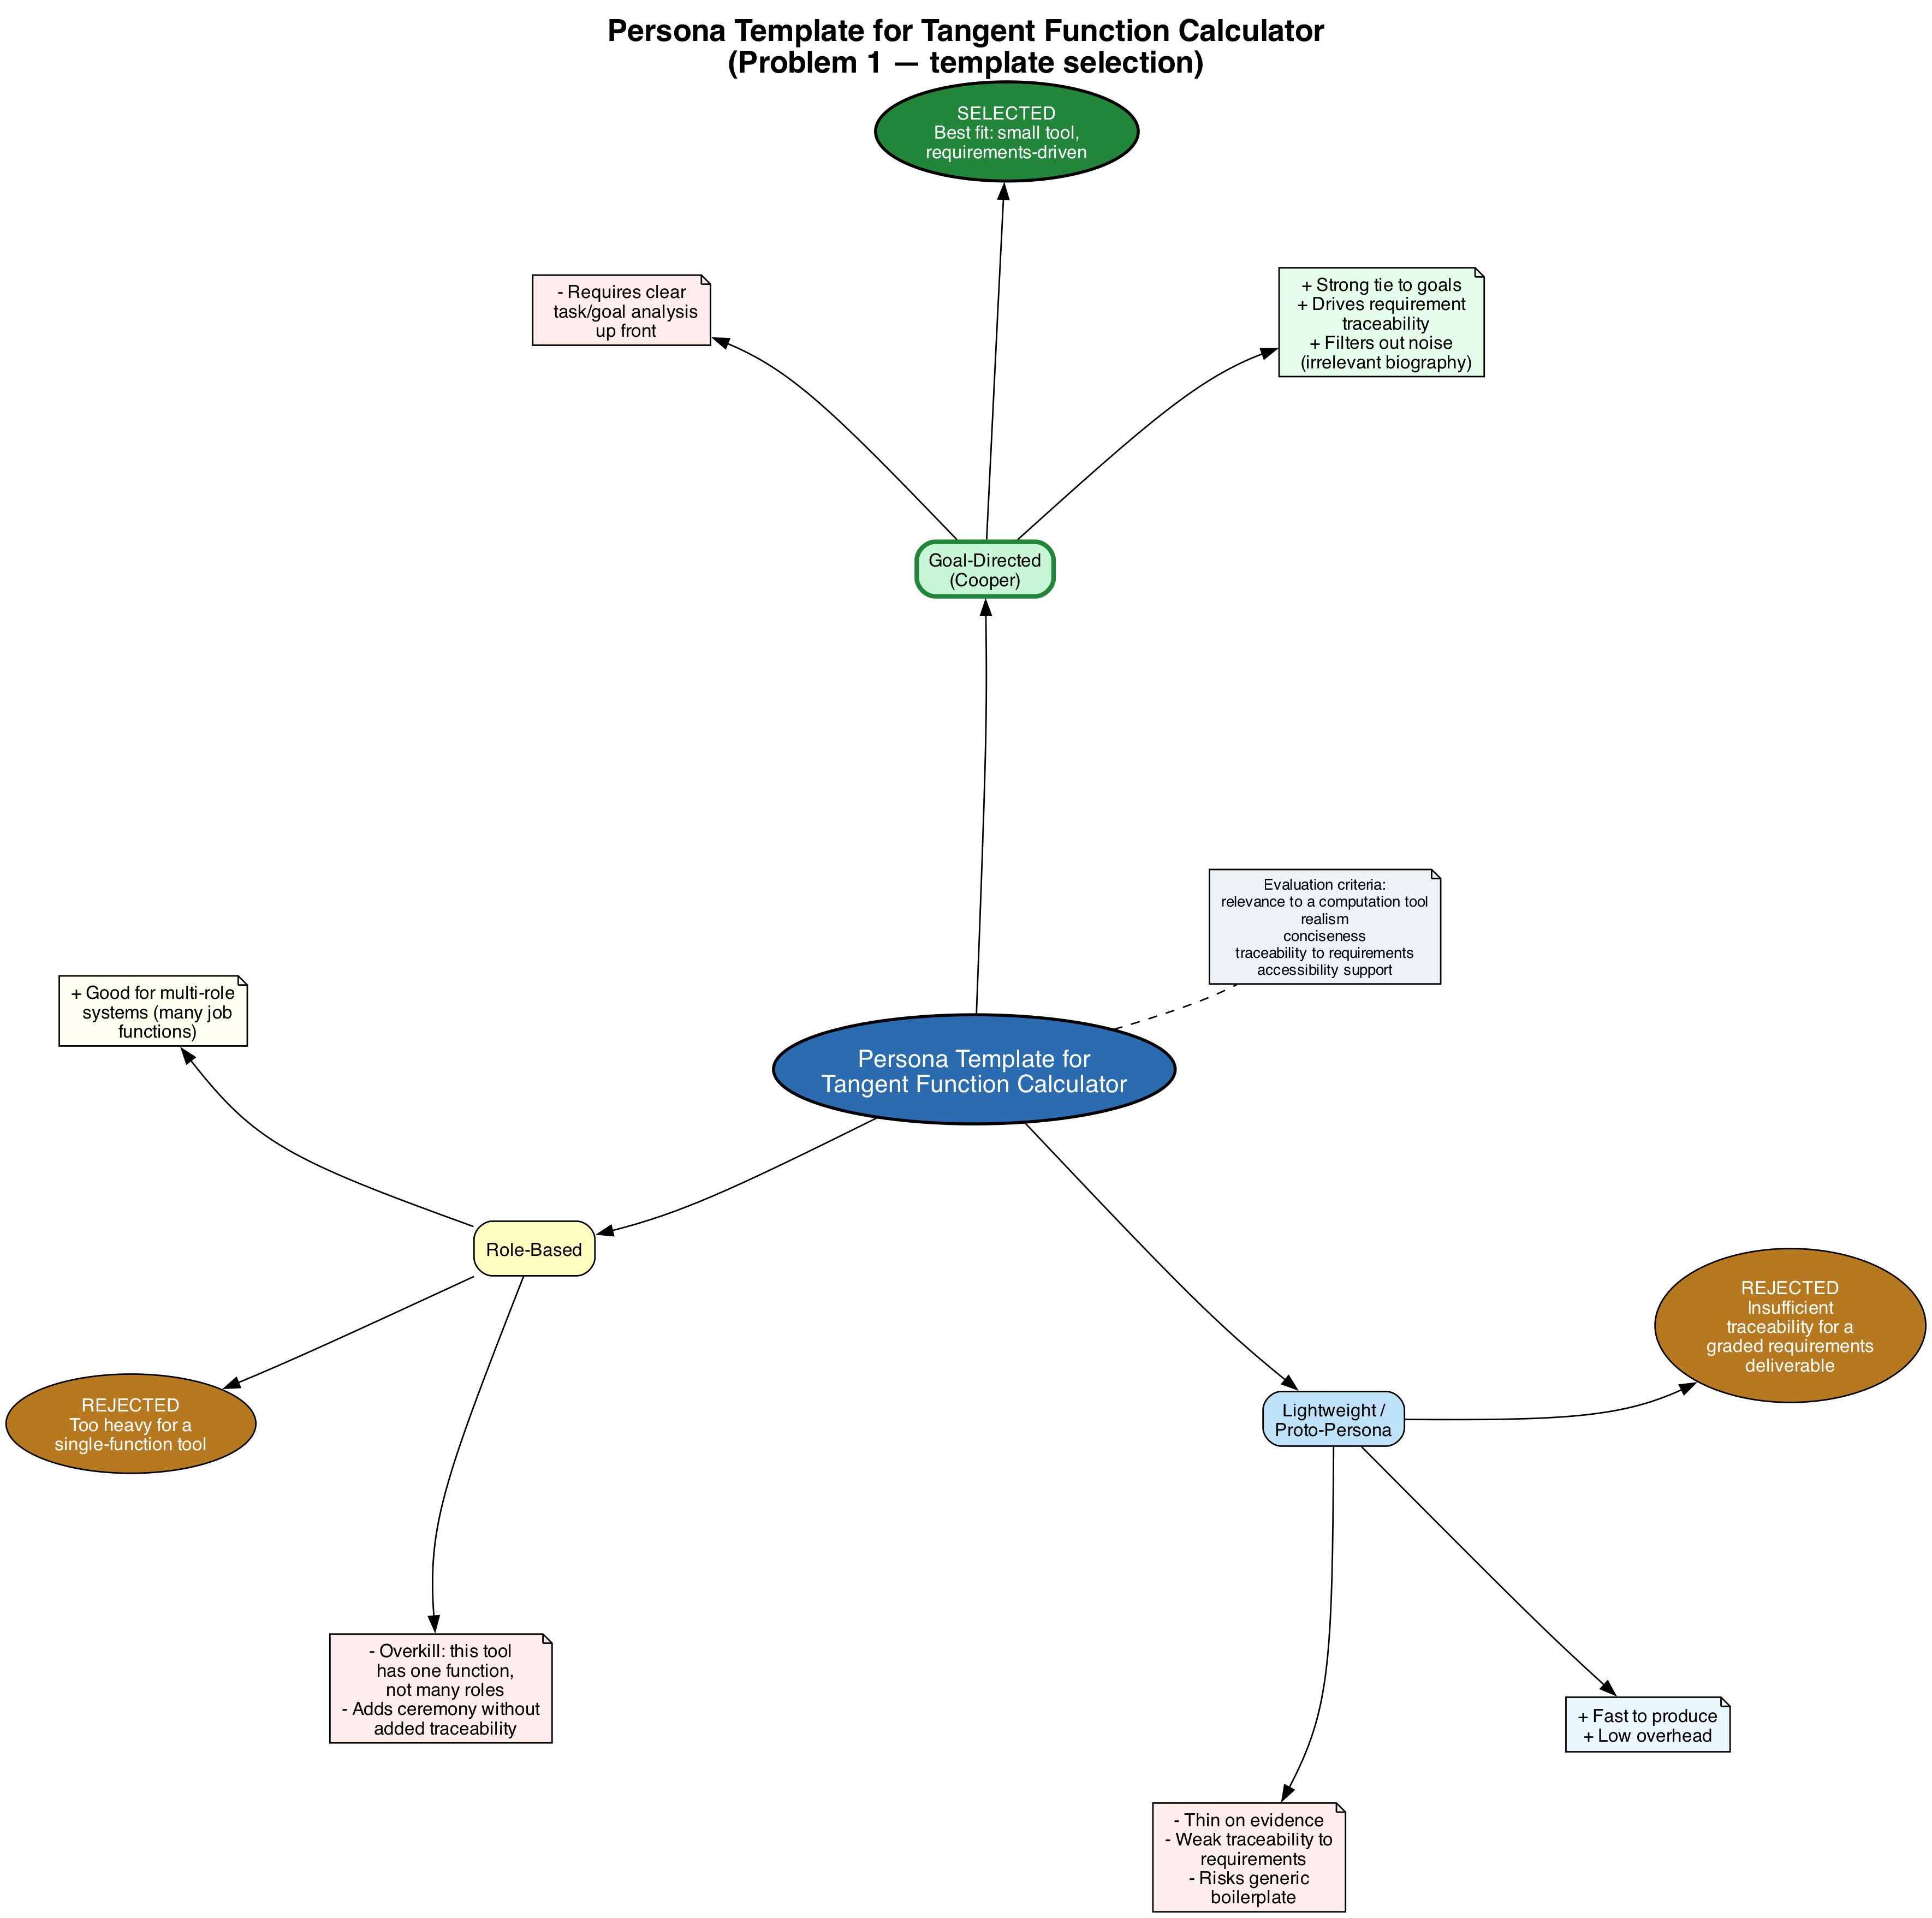
\includegraphics[width=\textwidth]{../../docs/mindmaps/persona_template_mindmap.png}
    \end{column}
  \end{columns}
\end{frame}

\begin{frame}{Problem 1 --- Persona: Maya Chen}
  \begin{itemize}
    \item \textbf{Role:} M.A.Sc. Mechanical Engineering student, optics-lab research assistant
    \item \textbf{Goal:} a quick, trustworthy $\tan(x)$ value without opening a full CAS
    \item \textbf{Pain points:} radians/degrees confusion; distrust of results near $\pi/2$; no patience for raw tracebacks
  \end{itemize}
  \vspace{0.2cm}
  \textbf{7 traceable needs} identified (gate: $\ge 5$) $\to$ directly drive the Problem 2 requirements.
\end{frame}

\section{Requirements}
\begin{frame}{Problem 2 --- Requirements (ISO/IEC/IEEE 29148)}
  18 requirements, categories: \texttt{FR VAL ACC USE REL ERR DOC}. Each has an ID, statement, persona-traced rationale, priority, verification method.
  \begin{table}
    \footnotesize
    \begin{tabular}{@{}p{1.3cm}p{7.7cm}p{1cm}@{}}
      \toprule
      ID & Statement & Pri. \\
      \midrule
      VAL-03 & Reject input whose $|x|$ exceeds the documented maximum ($10^4$ rad); report the input as out of the supported range. & Must \\
      VAL-04 & Detect input $x$ within a documented tolerance of a pole ($x = \pi/2 + k\pi$) and treat it as an invalid computation rather than returning a numeric value. & Must \\
      ACC-01 & For accepted $x$ outside the pole-tolerance band and within the supported range, compute $\tan(x)$ with relative error $\le 10^{-9}$ vs.\ trusted reference values. & Must \\
      ERR-01 & When input is rejected under any VAL requirement, display a message identifying the specific condition violated. & Must \\
      \bottomrule
    \end{tabular}
  \end{table}
  \textbf{Quality review} caught 3 issues: an unquantified term ("fast and accurate"), an algorithm prescribed too early, a non-singular requirement -- all corrected before freezing \textbf{Baseline v0.1}.
\end{frame}

\section{Algorithms}
\begin{frame}[fragile]{Problem 3 --- Algorithm A: Range Reduction + Maclaurin Series}
  \begin{columns}
    \begin{column}{0.55\textwidth}
      \begin{lstlisting}[style=pseudo]
k <- ROUND(x / (PI/2))
r <- x - k*(PI/2)        // r in [-pi/4,pi/4]
sinR <- MACLAURIN-SIN(r)
cosR <- MACLAURIN-COS(r)
if |cosR| < EPSILON
    signal POLE-ERROR
return sinR / cosR
      \end{lstlisting}
    \end{column}
    \begin{column}{0.45\textwidth}
      \textbf{Convergence:} super-linear, $\sim$10--15 terms for $10^{-12}$ \\[0.2cm]
      \textbf{Trace:} $\tan(\pi/4)=1$ confirmed \\[0.2cm]
      \textbf{Weakness:} reduction error grows with $|x|$
    \end{column}
  \end{columns}
\end{frame}

\begin{frame}[fragile]{Problem 3 --- Algorithm B: CORDIC (Circular, Rotation Mode)}
  \begin{columns}
    \begin{column}{0.55\textwidth}
      \begin{lstlisting}[style=pseudo]
vx <- 1 ; vy <- 0 ; z <- r
for i <- 0 to N_MAX - 1
    if z >= 0 : d <- +1  else d <- -1
    vx_next <- vx - d*vy*2^(-i)
    vy_next <- vy + d*vx*2^(-i)
    z <- z - d*A[i]      // A[i]=arctan(2^-i)
    vx <- vx_next ; vy <- vy_next
if |vx| < EPSILON
    signal POLE-ERROR
return vy / vx           // K cancels for tan
      \end{lstlisting}
    \end{column}
    \begin{column}{0.45\textwidth}
      \textbf{Convergence:} linear, $\sim$1 bit/iteration, $\sim$40 iterations for $10^{-12}$ \\[0.2cm]
      \textbf{Trace:} $\tan(\pi/4)=1$ confirmed (0.986 after 7 iters $\to$ 1.000000000000 after 39) \\[0.2cm]
      \textbf{Weakness:} finite table precision caps ultimate accuracy
    \end{column}
  \end{columns}
\end{frame}

\section{Selection \& CLI}
\begin{frame}{Problem 4 --- Algorithm Selection}
  \begin{columns}
    \begin{column}{0.55\textwidth}
      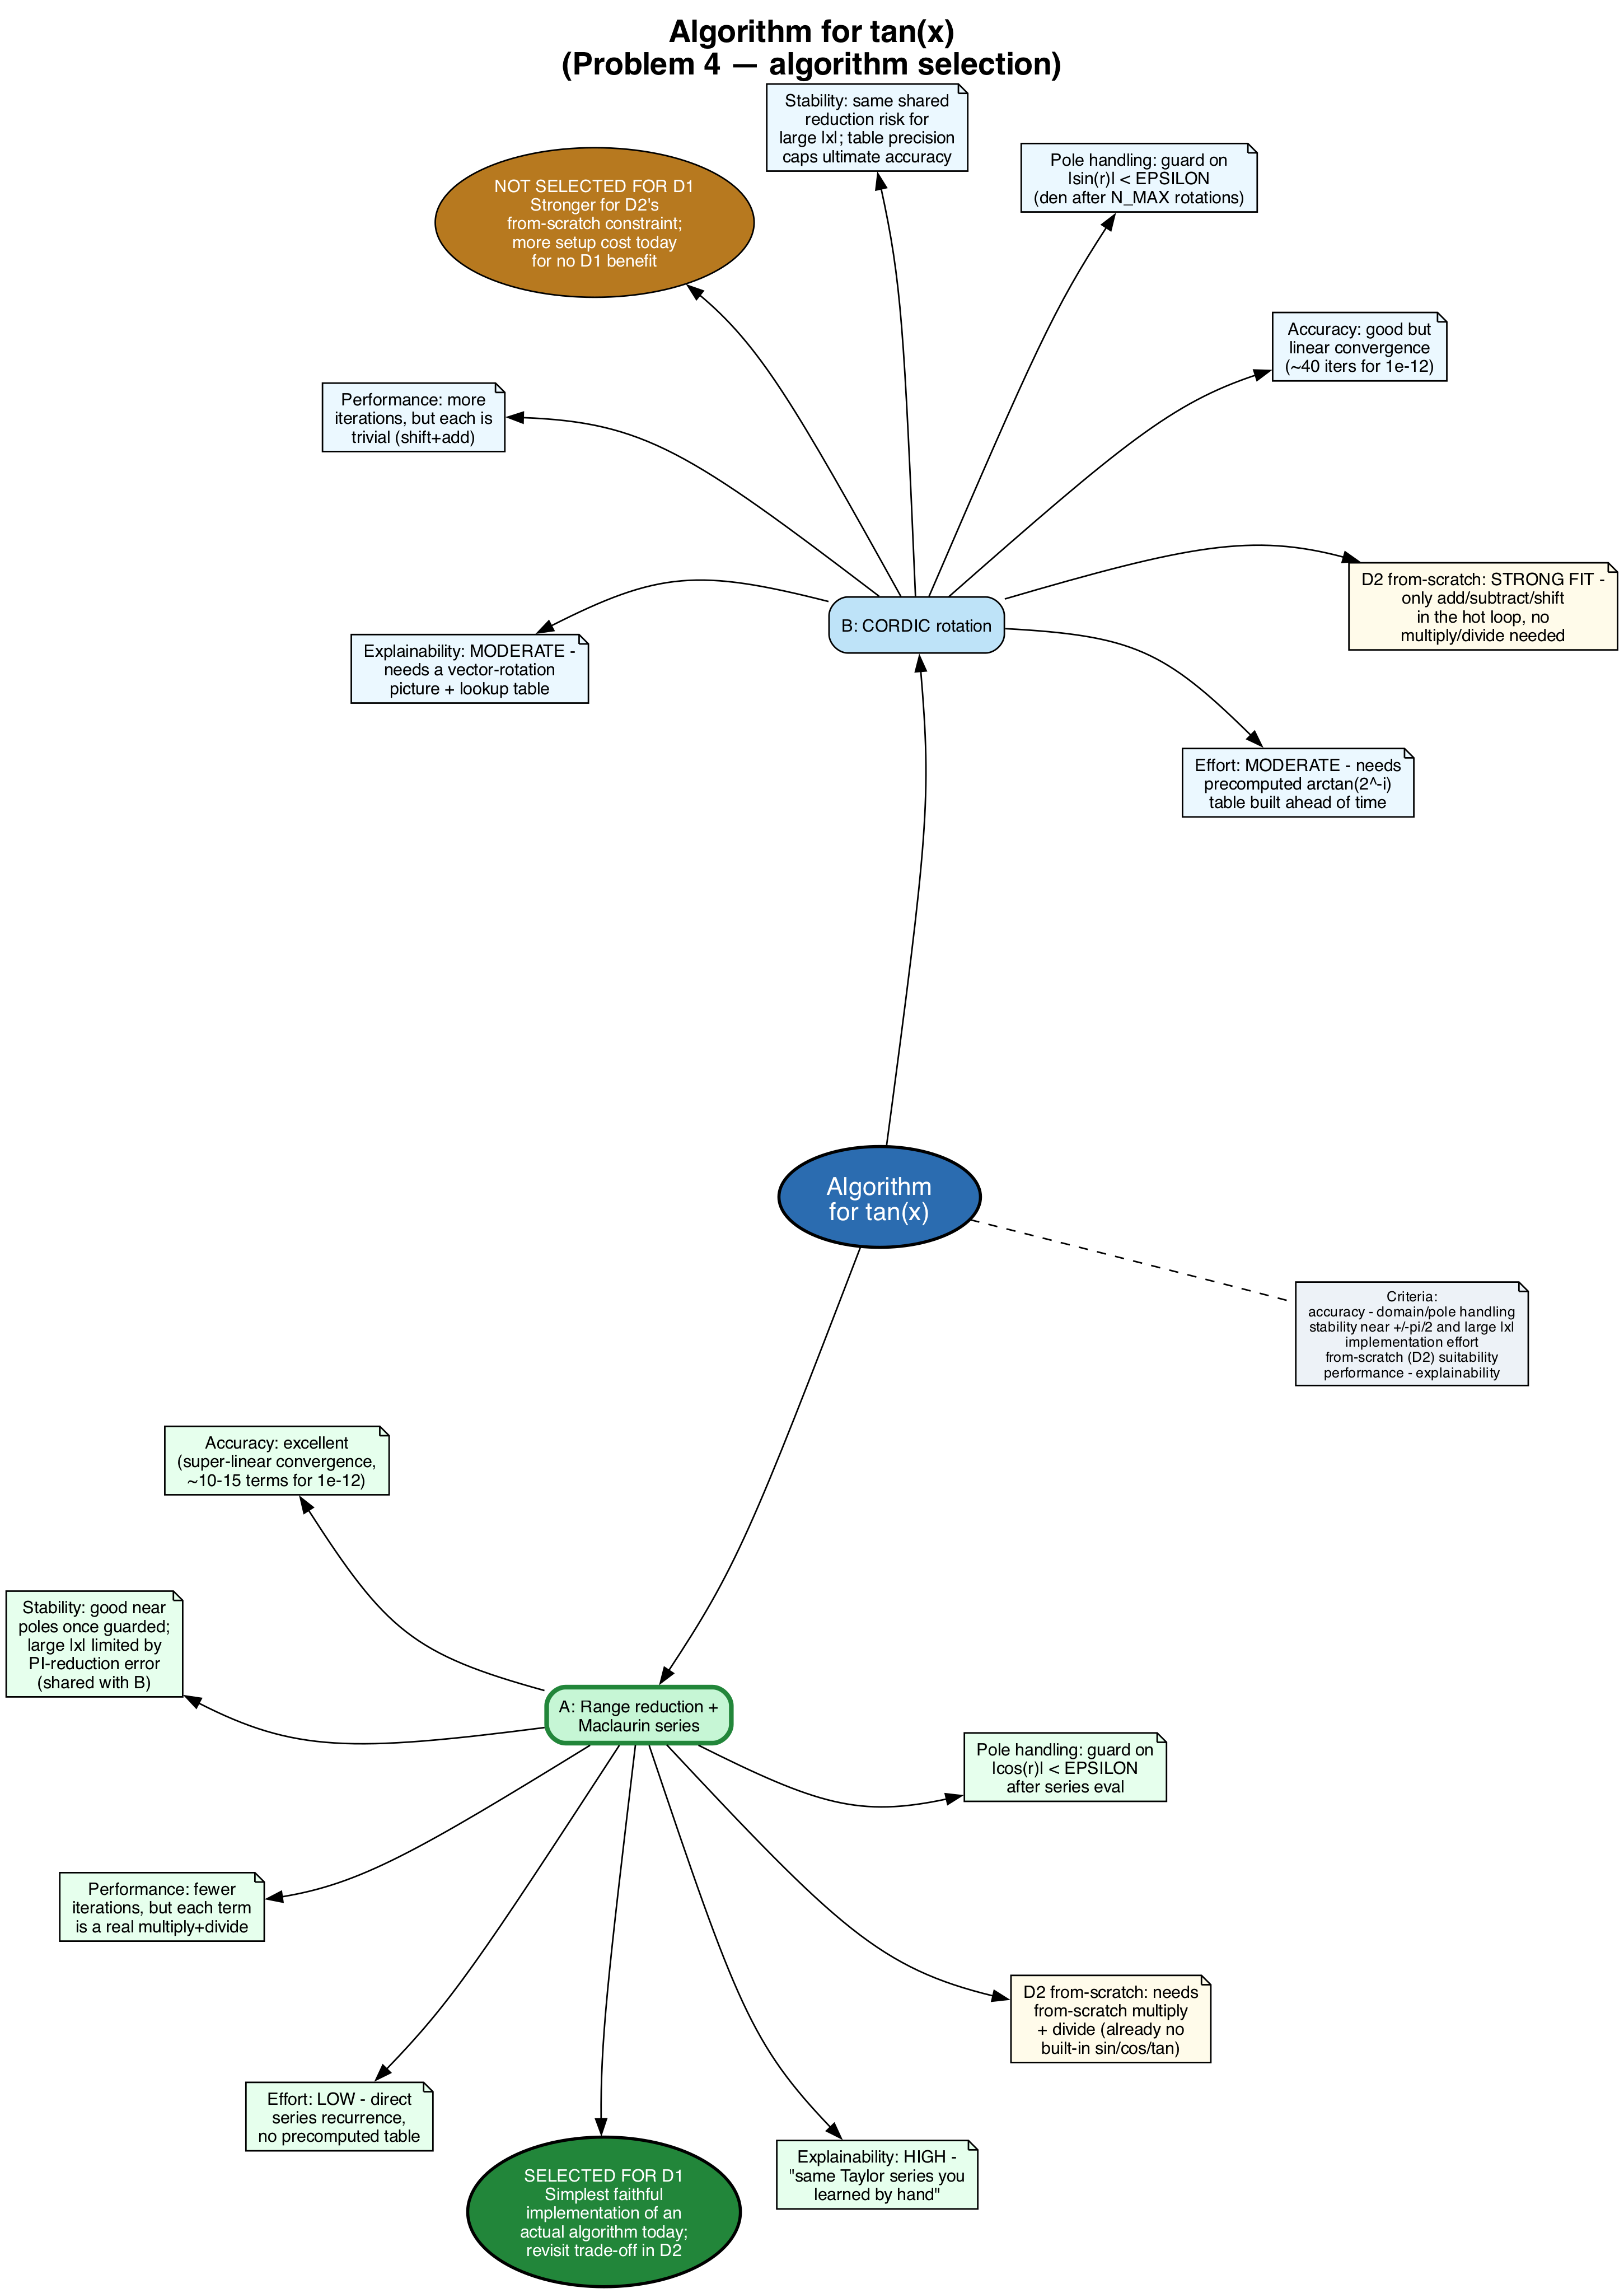
\includegraphics[width=\textwidth,height=0.75\textheight,keepaspectratio]{../../docs/mindmaps/algorithm_selection_mindmap.png}
    \end{column}
    \begin{column}{0.45\textwidth}
      \textbf{Selected: Algorithm A} for the D1 prototype.

      \vspace{0.2cm}
      Lowest implementation effort, most explainable to the persona.

      \vspace{0.2cm}
      Algorithm B (CORDIC) noted as the stronger candidate for D2's from-scratch, multiplication-free constraint -- revisit then.
    \end{column}
  \end{columns}
\end{frame}

\begin{frame}{Problem 4 --- CLI Prototype (\texttt{src/cli.py})}
  \begin{itemize}
    \item Compute layer (\texttt{maclaurin\_sin/cos}, \texttt{tan\_by\_series}) separated from I/O layer
    \item Two custom exceptions: \texttt{OutOfRangeError}, \texttt{NearPoleError}
    \item States angle unit + domain hint before first prompt; 10 significant figures displayed
  \end{itemize}
\end{frame}

\begin{frame}{Live Demo / Sample Runs}
  \centering
  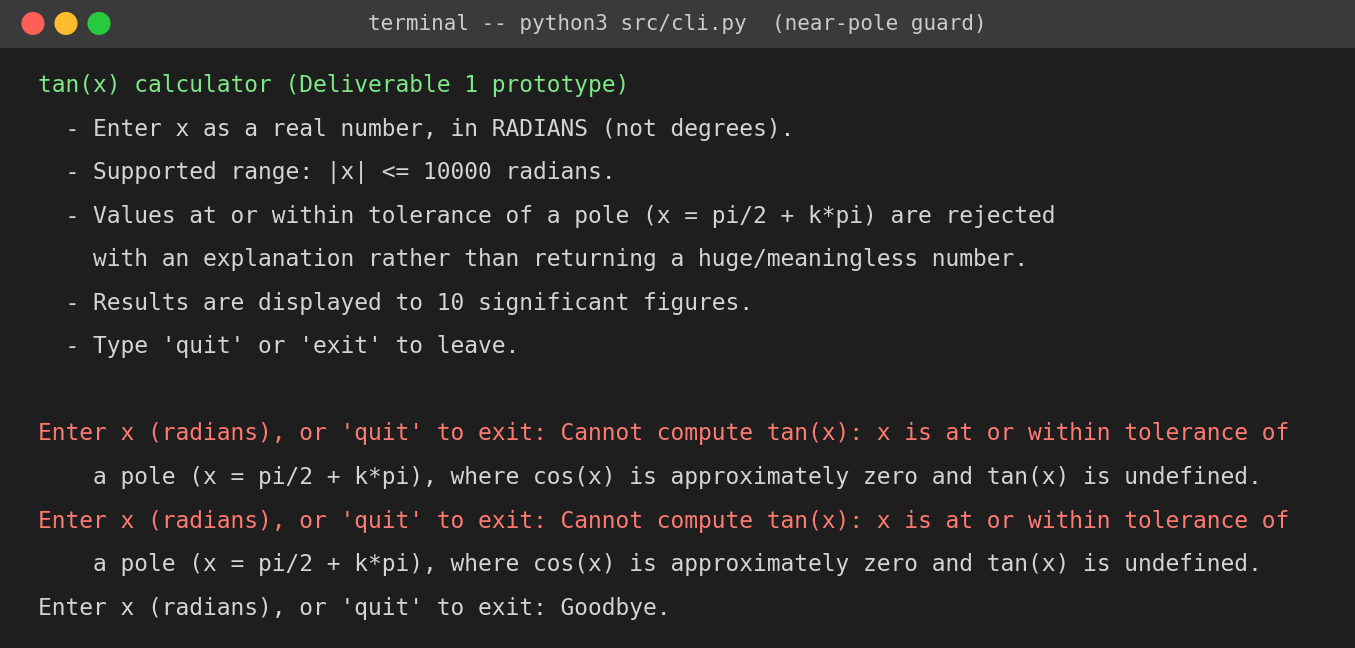
\includegraphics[width=0.72\textwidth]{../../docs/screenshots/run3_near_pole.png}
\end{frame}

\section{Verification \& Limitations}
\begin{frame}{Verification Highlights}
  \begin{table}
    \small
    \begin{tabular}{lll}
      \toprule
      Case & Result & Verdict \\
      \midrule
      $x=\pi/4$ & $\tan = 1$ & Pass \\
      $x=-\pi/4$ & $\tan = -1$ (odd symmetry) & Pass \\
      $x=\pi/2 - 10^{-9}$ & rejected (near-pole) & Pass \\
      $x = 1000$ & $1.470324156$, matches \texttt{math.tan} & Pass \\
      $x = 10^{10}$ & rejected (out of range) & Pass \\
      \bottomrule
    \end{tabular}
  \end{table}
  All demo cases traced to a requirement ID; full matrix in \texttt{docs/verification\_matrix.md}.
\end{frame}

\begin{frame}{Known Limitations}
  \begin{itemize}
    \item Large-argument accuracy degrades gradually below $|x|\le 10^4$; exact threshold not yet quantified
    \item Pole tolerance ($10^{-6}$) and $X\_MAX$ ($10^4$) are provisional, pending professor confirmation
    \item No performance/timing requirement verified (deliberately deferred)
    \item Reference values rely on \texttt{math.tan} (finite precision), adequate here but not an arbitrary-precision oracle
  \end{itemize}
\end{frame}

\section{GAI Prompts}
\begin{frame}{GAI Prompt --- Problem 1 (Persona)}
  \footnotesize
  \textbf{Tool:} Claude Code (Sonnet 5) \quad \textbf{Type:} Generative + decision-support
  \begin{description}
    \item[TASK] Compare $\ge 3$ persona-template styles (goal-directed, role-based, lightweight/proto) for a $\tan(x)$ calculator user as a mind-map outline; recommend one; then draft one persona (name, role, experience, skills, goals, environment, tan-specific needs/pain points) + usage scenario.
    \item[RESTRICTIONS] No invented statistics or real-person claims; every attribute must trace to $\ge 5$ later requirements; no implementation technology prescribed.
    \item[OUTPUT FORMAT] (1) template-comparison mind map + decision; (2) persona card + assumptions + 3--5 sentence usage scenario.
    \item[AUDIENCE] SOEN 6011 professor/TAs/grad SE students -- evidence-based, traceable to requirements.
  \end{description}
\end{frame}

\begin{frame}{GAI Prompt --- Problem 2 (Requirements)}
  \footnotesize
  \textbf{Tool:} Claude Code (Sonnet 5) \quad \textbf{Type:} Generative + transformational, with review
  \begin{description}
    \item[TASK] Express requirements per ISO/IEC/IEEE 29148 style, informed by the finalized Problem 1 persona; ID scheme FR/VAL/ACC/USE/REL/PERF/ERR/DOC; cover accepting $x$, angle unit, computing/displaying $\tan(x)$, clear/retry/exit, rejecting invalid/near-pole/extreme inputs, a measurable accuracy tolerance; list assumptions separately; review the draft against the 29148 quality characteristics.
    \item[RESTRICTIONS] No algorithm/library/language prescribed inside a requirement; no vague unquantified terms; each requirement singular and independently verifiable.
    \item[OUTPUT FORMAT] Requirements table (ID, Statement, Rationale/persona trace, Priority, Verification) + Assumptions list + Review-findings table.
    \item[AUDIENCE] Same -- standard-aligned, testable, traceable.
  \end{description}
\end{frame}

\begin{frame}{GAI Prompt --- Problem 3 (Two Algorithms)}
  \footnotesize
  \textbf{Tool:} Claude Code (Sonnet 5) \quad \textbf{Type:} Generative + comparative
  \begin{description}
    \item[TASK] Specify two independent, language-neutral algorithms in established pseudocode for $\tan(x)$, satisfying pasted Problem 2 requirement IDs (ACC-01, VAL-03, VAL-04, REL-01). Algorithm A: range reduction (period $\pi$, odd symmetry) + Maclaurin series for $\sin/\cos$. Algorithm B: CORDIC rotation (precomputed $\arctan(2^{-i})$ table). For each: inputs/outputs/pre-postconditions/constants/validation/stopping condition/max-work safeguard/complexity/weaknesses/worked trace.
    \item[RESTRICTIONS] No real programming-language syntax; every loop must terminate or have a max-work cap; no built-in $\sin/\cos/\tan$ assumed; algorithms must be genuinely different.
    \item[OUTPUT FORMAT] Two pseudocode listings, each with pre/post note, complexity/limitations note, worked trace; "How A and B differ" comparison table.
    \item[AUDIENCE] Same -- rigorous, unambiguous, independently implementable.
  \end{description}
\end{frame}

\begin{frame}{GAI Prompt --- Problem 4 (Selection + CLI)}
  \footnotesize
  \textbf{Tool:} Claude Code (Sonnet 5) \quad \textbf{Type:} Decision-support + generative
  \begin{description}
    \item[TASK] Step 1: mind-map comparing the two Problem 3 algorithms on accuracy, domain/pole handling, stability, effort, D2 from-scratch suitability, performance, explainability; select one, justify rejecting the other. Step 2: Python 3 CLI implementing the selected algorithm; separate I/O from compute; prompt for $x$ + angle unit + domain hint; validate; detect near-pole; compute; display with documented precision; catch invalid/numerical-failure cases.
    \item[RESTRICTIONS] Selection must follow the stated criteria and anticipate the D2 from-scratch constraint; must run from a terminal with no unhandled traceback on invalid/near-pole input; compute core independently callable; may use Python's \texttt{math} in D1, but note which calls need from-scratch replacement in D2.
    \item[OUTPUT FORMAT] (1) selection mind map + decision; (2) full Python source; (3) sample runs (valid/near-pole/negative/invalid) + command used.
    \item[AUDIENCE] Same -- evidence-based selection, clean/robust code, runnable outside an IDE.
  \end{description}
\end{frame}

\section{References}
\begin{frame}{References}
  \small
  \begin{itemize}
    \item A. Cooper et al., \emph{About Face 3}. Wiley, 2007.
    \item J. Pruitt, T. Adlin, \emph{The Persona Lifecycle}. Morgan Kaufmann, 2006.
    \item ISO/IEC/IEEE 29148:2018, Requirements Engineering.
    \item J. E. Volder, ``The CORDIC Trigonometric Computing Technique,'' \emph{IRE Trans.\ Electronic Computers}, 1959.
    \item J.-M. Muller et al., \emph{Handbook of Floating-Point Arithmetic}, 2nd ed., 2016.
    \item T. Cormen et al., \emph{Introduction to Algorithms}, 3rd ed., MIT Press, 2009.
    \item NIST Digital Library of Mathematical Functions, \url{https://dlmf.nist.gov/}.
  \end{itemize}
\end{frame}

\begin{frame}{Thank You}
  \centering
  \Large Questions?
\end{frame}

\end{document}
